\chapter{계보: biological replay에서 multi-rate neural memory까지}
\label{STC-S05}

Sleep-time compute는 2026년에 갑자기 생긴 단일 논문 계열이 아니다. Fast/slow learning theory,
continual learning, generative replay, external agent memory, test-time neural memory, asynchronous
memory agents가 서로 다른 문제를 풀다가 하나의 lifecycle로 수렴한다.

\begin{figure}[htbp]
  \centering
  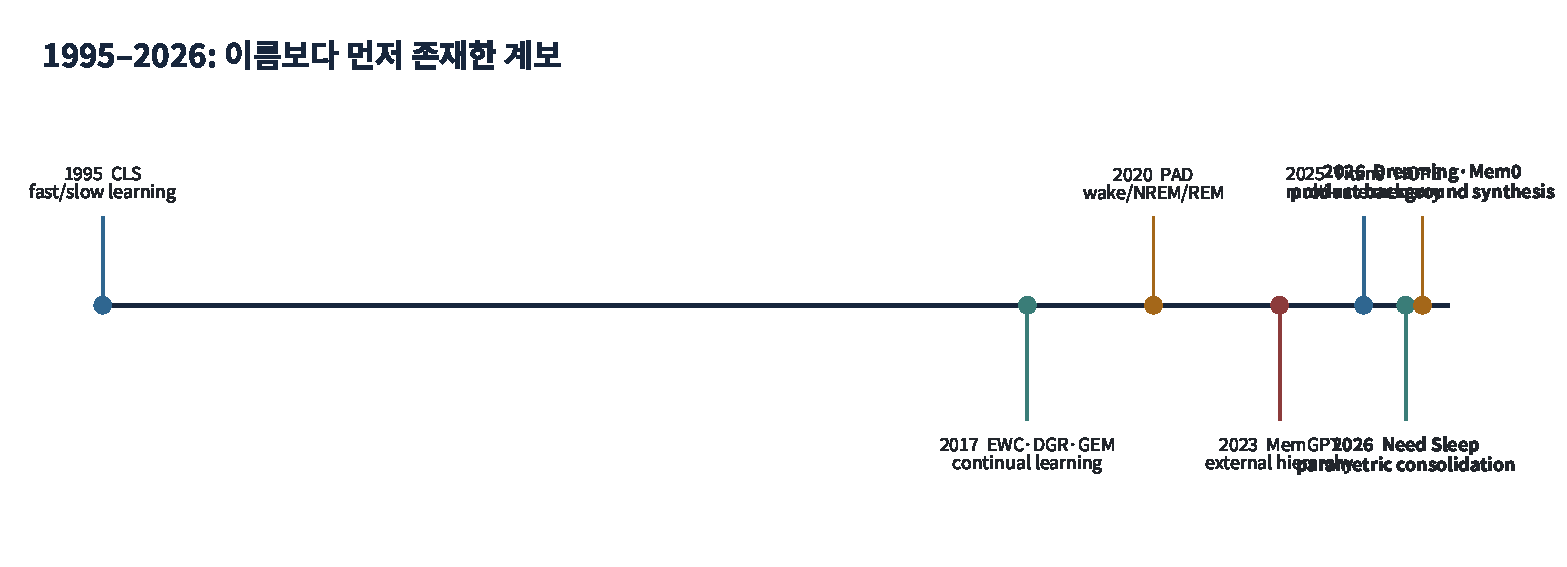
\includegraphics[width=0.98\textwidth]{figures/stc-f003.pdf}
  \caption{1995–2026 evidence chronology. 연도는 공개 source의 최초 publication/release 기준이며,
  같은 시기의 방법이 동일 maturity라는 뜻은 아니다.}
  \stcfigure{STC-F003}
  \figsource{Original synthesis; SRC-STC-0001--SRC-STC-0063}{1995 CLS에서 2017 continual learning, 2020 PAD, 2023 MemGPT, 2025 Titans/HOPE, 2026 parametric sleep과 product dreaming으로 이어지는 시간축.}
  \label{fig:stc-chronology}
\end{figure}

\section{1995: complementary learning systems}

CLS는 hippocampus의 빠른 episodic acquisition과 neocortex의 느린 interleaved learning을 분리했다
\parencite{srcstc0001}. 이 관점이 제공하는 basis는 ``새 기억을 빠르게 받는 store''와 ``기존 구조를
보존하며 천천히 통합하는 learner''를 한 update rule로 강제하지 않는다는 점이다. 오늘의 system으로
번역하면 wake log/episodic memory와 sleep consolidation model의 역할 분리다.

그러나 biology에서 production architecture를 곧바로 도출할 수는 없다. Biological model은 user
scope, exact delete, source attribution, model release compatibility를 다루지 않는다. 따라서 계보는
mechanism inspiration이지 deployment evidence가 아니다.

\section{2017: continual-learning baselines가 먼저 만든 consolidation 문제}

Deep Generative Replay는 generator의 pseudo-data와 새 data를 함께 학습해 과거 task forgetting을 줄이는
강한 non-sleep-named baseline이다.\claim{STC-C019} \parencite{srcstc0003} EWC는 이전 task에 중요한
parameter를 Fisher-weighted quadratic penalty로 보호해 stability와 plasticity를 trade-off한다.
\claim{STC-C020} \parencite{srcstc0002} GEM은 stored examples의 gradient를 constraint로 사용해 이전
task loss가 국소적으로 증가하지 않게 update를 투영한다.\claim{STC-C021} \parencite{srcstc0004}

Progress \& Compress는 active column에서 새 task를 배우고 consolidation phase에서 knowledge base로
압축하는 periodic-refresh 대안을 제시했다.\claim{STC-C022} \parencite{srcstc0007} 이 계열은 중요한
교훈을 준다. ``Sleep''이라는 이름 없이도 progress/online phase와 compress/offline phase를 나눌 수
있으며, 새 term의 가치는 matched resource에서 기존 periodic consolidation보다 나아야 한다.

\section{2020–2022: NREM/REM analogy를 계산 mechanism으로 만든 연구}

PAD(Perturbed and Adversarial Dreaming)는 wake, NREM-like perturbed replay, REM-like adversarial dreaming을
분리해 cortical representation learning을 연구했다.\claim{STC-C018} \parencite{srcstc0009}
Hippocampus--neocortex computational model은 autonomous offline dynamics와 alternating NREM/REM regime로
새 정보 통합과 old knowledge 보호를 함께 탐구했다.\claim{STC-C017} \parencite{srcstc0010}

2022년 PLOS Computational Biology의 spiking-network 연구는 두 task 설정에서 interleaved sleep-like
replay가 joint synaptic representation을 형성하고 catastrophic forgetting을 줄였다고 보고했다.
\claim{STC-C016} \parencite{srcstc0011} 이것은 user-scale LLM deployment 증거가 아니라, online data 없이
autonomous replay가 consolidation을 도울 수 있다는 mechanism evidence다. Task 수, modality, network
scale, governance의 외삽을 분리해야 한다.

\section{2023–2025: external hierarchy와 wake-time neural memory}

MemGPT는 제한된 context와 external storage 사이에서 information을 paging하는 OS-style hierarchy로
long-term agent memory를 framing했다.\claim{STC-C011} \parencite{srcstc0013} 여기서 중요한 변화는
``모델이 모든 것을 weights에 기억해야 한다''에서 ``virtual memory처럼 context와 archival memory를
관리한다''로의 이동이다.

Titans는 surprise-driven update로 test time에 neural memory state를 학습하지만, 그 자체는 wake-path
fast-state learning이지 deferred cross-session sleep은 아니다.\claim{STC-C023}
\parencite{srcstc0017} 이 구분은 user framing의 핵심이다. Test-time learning은 current/near-current
stream에 적응하고, sleep-time learning은 더 넓은 replay와 검증을 거쳐 longer-lived state를 publish한다.

Nested Learning/HOPE는 optimization process를 여러 update frequency의 nested memory level로 보아
cadence를 분석하는 유용한 틀을 제공하지만, 공개 evidence는 deployed asynchronous sleep consolidation을
입증하지 않는다.\claim{STC-C024} \parencite{srcstc0020} HOPE의 CMS처럼 서로 다른 frequency로 갱신되는
state는 wake/sleep scheduler에 자연스럽게 매핑되지만, frequency hierarchy와 lifecycle publication은
별개 요구다.

\section{2026: 명시적 parametric sleep과 product synthesis의 분기}

2026년 계보는 둘로 갈라진다. 한쪽은 Language Models Need Sleep처럼 self-modification과 replay-like
training으로 parametric memory를 통합하는 연구다. 다른 쪽은 Dreaming, Mem0 Dream, Letta처럼 external
memory를 background에서 합성하는 product lifecycle이다. 두 방향은 같은 sleep boundary를 공유하지만
state medium과 evidence maturity가 다르다.

\begin{table}[htbp]
\centering
\caption{계보별 evidence가 실제로 지지하는 범위}
\label{tab:lineage-boundaries}
\small
\begin{tabularx}{\textwidth}{p{0.20\textwidth} X X}
\toprule
계보 & 지지하는 것 & 아직 지지하지 않는 것 \\
\midrule
biological/computational sleep & autonomous replay와 multi-phase integration 가능성 & LLM fleet economics, delete/rollback \\
continual learning & forgetting을 줄이는 replay·constraint·isolation mechanism & 무한 capacity, task-free production stability \\
external agent memory & bounded context 밖 persistent state와 hierarchy & parametric skill acquisition \\
neural/test-time memory & forward path에서 learned state update 가능성 & deferred multi-session publication \\
explicit parametric sleep & self-modification+consolidation research proof & broad per-user production deployment \\
product dreaming & scheduled external background synthesis & foundation-weight training 공개 증거 \\
\bottomrule
\end{tabularx}
\end{table}

\begin{keypoint}[계보의 종합]
새로운 것은 replay 자체가 아니라, persistent agent product가 wake-derived state를 background에서 계속
변환하며 serving lifecycle로 운영하기 시작했다는 점이다. 과학적 novelty는 matched alternative 대비
효과와 scaling surface에서, 산업적 novelty는 publication·rollback·memory plane의 지속 운영에서 평가한다.
\end{keypoint}
